\titre{ Loi d'un couple de variables aléatoires }
\theme{probabilités}
\auteur{}
\organisation{AMSCC}


\texte{ Soit $(X,Y)$ un couple de variables aléatoires admettant pour densité la fonction $f$ définie par 
	$$f(x,y) = k \cdot \textbf{1}_{\mathcal{C}}(x,y)$$
	où $\mathcal{C} = \{(x,y) \in \mathbb{R}^2 \mid |x|+|y| \leq 1 \}$ et $k \in \R$. }

\begin{enumerate}
	\item \question{ Dire lequel de ces trois domaines de $\R^2$ représentés ci-dessous est le domaine $\mathcal{C}$.
		
		\begin{minipage}{0.2\textwidth}
			\begin{center}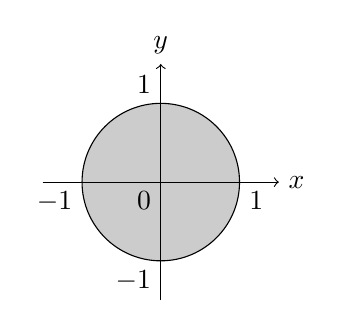
\begin{tikzpicture}
					\fill[gray!40] (0,0) circle (1);
					\draw (0,0) circle(1);	
					\draw[->] (-1.5,0) -- (1.5,0) node[right] {$x$};\draw[->] (0,-1.5) -- (0,1.5) node[above] {$y$};
					\draw[] (1,0) node[below right] {$1$};
					\draw[] (-1,0) node[below left] {$-1$};
					\draw[] (0,1) node[above left] {$1$};
					\draw[] (0,-1) node[below left]{$-1$};
					\node[below left] at (0,0) {$0$};
				\end{tikzpicture}\\ D1\end{center}
		\end{minipage}
		\hfill
		\begin{minipage}{0.2\textwidth}
			\begin{center}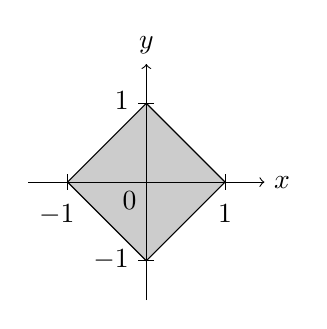
\begin{tikzpicture}
					\fill[gray!40] (-1,0) -- (0,1) -- (1,0) -- (0,-1) -- cycle;
					\draw (-1,0) -- (0,1) -- (1,0) -- (0,-1) -- cycle;
					\draw[->] (-1.5,0) -- (1.5,0) node[right] {$x$};\draw[->] (0,-1.5) -- (0,1.5) node[above] {$y$};\foreach \x in {-1} {\draw (\x,0.1cm) -- (\x,-0.1cm) node[below] {$\x\phantom{-}\strut$};}
					\foreach \x in {1,} {\draw (\x,0.1cm) -- (\x,-0.1cm) node[below] {$\x\strut$};}
					\foreach \y in {-1,1} {\draw (0.1cm,\y) -- (-0.1cm,\y) node[left] {$\y\strut$};}
					\node[below left] at (0,0) {$0$};	
				\end{tikzpicture}\\ D2\end{center}
		\end{minipage}
		\hfill
		\begin{minipage}{0.2\textwidth}
			\begin{center}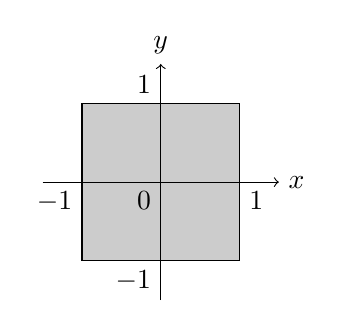
\begin{tikzpicture}
					\fill[gray!40] (-1,1) -- (1,1) -- (1,-1) -- (-1,-1) -- cycle;
					\draw (-1,1) -- (1,1) -- (1,-1) -- (-1,-1) -- cycle;
					\draw[->] (-1.5,0) -- (1.5,0) node[right] {$x$};
					\draw[->] (0,-1.5) -- (0,1.5) node[above] {$y$};
					\draw[] (1,0) node[below right] {$1$};
					\draw[] (-1,0) node[below left] {$-1$};
					\draw[] (0,1) node[above left] {$1$};
					\draw[] (0,-1) node[below left]{$-1$};
					\node[below left] at (0,0) {$0$};
				\end{tikzpicture}\\ D3\end{center}
	\end{minipage} }
	\reponse{Le domaine $\mathcal{C}$ est représenté en $D2$. C'est un carré d'aire = 2}
	
	\item \question{ Déterminer la valeur de $k \in \R$ telle que $f$ définisse bien une fonction densité. }
	
	\reponse{On choisit $k$ de telle sorte que $f \geq 0$ et $\iint f(x,y)dxdy = 1$. Or $\iint f(x,y)dxdy = k \iint_{\mathcal{C}} dxdy = k \times aire(\mathcal{C}) = 2k$. Donc il faut prendre \fbox{$k = \frac{1}{2}$}. 
		
		
		On peut aussi faire calcul de manière analytique en utilisant la relation de Chasles (on distingue selon le signe de $x$ et on encadre $y$) et le théorème de Fubini :
		
		
		\begin{align*}
			\iint_{\mathcal{C}} dxdy &= \int_{-1}^{0} \left( \int_{-1-x}^{1+x} dy\right)dx + \int_{0}^{1} \left( \int_{-1+x}^{1-x} dy\right)dx \\
			&= \int_{-1}^{0} \left( 2+2x\right)dx + \int_{0}^{1} \left(2-2x\right)dx \\
			&= 2 
		\end{align*}	
		
	}
	
	\item \question{ Déterminer les lois marginales du couple $(X,Y)$. }
	
	\reponse{On calcule les densités marginales : pour tout $x \in \R$ :
		Si $x >1$ ou si $x<-1$ : $f_X(x) = \int_\R f(x,y)dy = \int_\R 0 = 0$ ;
		
		Si $x \in [0;1]$ :
		\begin{align*}
			f_X(x) &= \int_\R f(x,y)dy \\
			&= \frac{1}{2}\int_{-1+x}^{1-x} dy \\
			&= 1-x
		\end{align*}
		
		Si $x \in [-1;0]$ :
		\begin{align*}
			f_X(x) &= \int_\R f(x,y)dy \\
			&= \frac{1}{2}\int_{-1-x}^{1+x} dy \\
			&= 1+x
		\end{align*}
		
		Avec des fonctions indicatrices, cela se réécrit pour tout $x \in \R$ :
		
		$$f_X(x) = \textbf{1}_{[-1;0[}(x)(1+x) + \textbf{1}_{[0;1[}(x)(1-x) = \textbf{1}_{[-1;1]}(x)(1-|x|) $$
		
		Les rôles étant symétriques en $x$ et en $y$, on obtient de manière similaire que pour tout $y \in \R$ : $$f_Y(y) = \textbf{1}_{[-1;0[}(y)(1+y) + \textbf{1}_{[0;1[}(y)(1-y) = \textbf{1}_{[-1;1]}(y)(1-|y|)$$}
	\item \question{ Déterminer $cov(X,Y)$. }
	
	\reponse{On utilise la formule de Huygens : $cov(X,Y) = \mathbb{E}(XY)-\mathbb{E}(X)\mathbb{E}(Y)$. 
		Ainsi, on calcule :
		\begin{align*}
			\mathbb{E}(X) &= \int_\R xf_X(x)dx \\
			&= \int_{-1}^{0} x(1+x)dx + \int_{0}^{1} x(1-x)dx \\
			&= -\frac{1}{6}+\frac{1}{6} \\
			&=0
		\end{align*}
		
		Du fait que $X$ et $Y$ suivent la même loi, on déduit que $\mathbb{E}(Y) = 0$.
		
		Il reste à calculer :
		\begin{align*}
			\mathbb{E}(XY) &= \iint_{\R^2} xyf(x,y)dxdy \\
			&= \frac{1}{2}\iint_{\mathcal{C}} dxdy \\
			&= \frac{1}{2}\int_{-1}^{0} \left( \int_{-1-x}^{1+x} xydy\right)dx + \frac{1}{2}\int_{0}^{1} \left( \int_{-1+x}^{1-x} xydy\right)dx \\ 
			&= \frac{1}{2}\int_{-1}^{0} x \left[\frac{y^2}{2}\right]_{-1-x}^{1+x} dx + \frac{1}{2}\int_{0}^{1}   x\left[\frac{y^2}{2}\right]_{-1+x}^{1-x}dydx \\ 
			&= \frac{1}{2}\int_{-1}^{0} (x \times 0) dx + \frac{1}{2}\int_{0}^{1}   (x \times 0) dx \\
			&= 0
		\end{align*}
		
		On en déduit que $\fbox{cov(X,Y) = 0}$. 
	}
	
	\item \question{ \'Etudier l'indépendance des variables $X$ et $Y$. }
	
	\reponse{On pourrait penser que les variables sont indépendantes car leur covariance est nulle. Cependant, ce n'est pas une condition suffisante et on observe que $f_X(x)f_Y(y) \neq f(x,y)$.
		La conclusion est que \fbox{$X$ et $Y$ ne sont pas indépendantes}.  }
\end{enumerate}